\section{Применение ``CATIA-GDML geometry builder'' к CBM RICH}\label{sec:RICHgeo}

Значительная часть работы над ``Builder'' выполнялась при поддержке группы CBM RICH, поэтому самая сложная MC-модель построенная с помощью ``Builder'' это CBM RICH. Построенная за несколько итераций модель имеет достаточно сложную иерархию и характеризуется высокой степенью подробностей.

Для того, чтобы GDML без проблем импортировался в CbmRoot было написано дополнение.

Геометрическая MC-модель детектора RICH эксперимента CBM имеет многоуровневую структуру, в основном обоснованную физической структурой сборки, но иногда и \todo бывает неочевидной и неестественной с целью повышения эфективности проведения частиц.

На момент написания данной работы инженерный проект не был завершён --- некоторые узлы были проработаны достаточно подробно и прошли несколько этапов уточнения, в которых модель менялась принципиально. В то же время некоторые узлы существуют лиш на концептуальном уровне. В первую очередь к ним относится форма и конструкция корпуса детектора, проектирование которой не составляет особого труда и может быль отложена на более поздний этап. Большая часть корпуса не оказывает влияния на эффективность детектора, т.к. лежит за пределами геометрического аксептанса, поэтому допускается моделирование физики детектора с упрощённой моделью корпуса, либо вообще без него.

В детекторе RICH можно выделить несколько подсистем --- фоточувствительная камера, магнитный экран вокруг камеры, зеркала, система опор зеркал, часть ионопровода в RICH, корпус детектора. Рассмотрим реализацию каждой подсистемы в MC-модели, построенной с помощью ``CATIA-GDML geometry builder''.

\subsection{Фоточувствительная камера}\label{sec:RICHgeoCamera}

Планируется, что фоточувствительная камера CBM RICH будет составлена из модулей, содержащих 2$\times$3 МА~ФЭУ Hamamatsu H12700, см. \figref{fig:H12700drawing}. Один такой МА~ФЭУ имеет габариты 52$\times$52~мм$^2$, между МА~ФЭУ оставляется зазор 1~мм для запаса по точности, таким образом размер модуля составляет 158мм$\times$105мм.

\begin{figure}[H]
\centering
\includegraphics[width=0.7\textwidth]{pictures/H12700_drawing.png}
\caption{Чертёж МА~ФЭУ H12700 из документации.}
\label{fig:H12700drawing}
\end{figure}

В момент написания данной работы ведётся работа по проектированию модуля, разработке программ для FPGA, но имеются изготовленный прототип. Помимо МА~ФЭУ в модуль входят 12~плат передней электроники DIRICH, одна плата, обеспечивающая питание, и одна плата концентрации данных. В основе модуля лежит плата-адаптер, к которой с одной стороны подсоединяются МА~ФЭУ, а с другой --- все платы. CAD-модель и MC-модель модуля показаны на \figref{fig:geoMCmodule}.

\begin{figure}[H]
\begin{minipage}[b]{0.495\textwidth}
\includegraphics[width=1.0\textwidth]{pictures/PMTmoduleCAD.png}
\end{minipage}
\hspace{0.01\textwidth}
\begin{minipage}[b]{0.495\textwidth}
\includegraphics[width=1.0\textwidth]{pictures/Module_1_cut.png}
\end{minipage}
\caption{CAD-модель (слева) и MC-модель (справа) модуля фоточувствительной камеры CBM RICH.}
\label{fig:geoMCmodule}
\end{figure}

%Пиксели
%№№ 2-7, 58-63, 9, 17,..., 49, 16, 24,..., 56
МА~ФЭУ моделируется до уровня пикселей. Это позволяет максимально приблизить моделирование прохождения частиц в CbmRoot и обработку реальных данных. В соответствии с документацией, у МА~ФЭУ H12700 пиксели имеют разные размеры (см. \figref{fig:H12700drawing}): угловые пиксели (№№ 1, 8, 57, 64) 6.25мм$\times$6.25мм, пиксели по краям, кроме угловых, --- 6.25мм$\times$6мм, остальные, центральные пиксели --- 6мм$\times$6мм. Для того, чтобы представить три типа пикселей в MC-модели, необходимо три отдельных объёма, имеющих разную форму. Чтобы сделать модель максимально понятной и гибкой принято решение отделить пиксели из крайних горизонтальных рядов от пикселей из крайних вертикальных рядов и моделировать их с помощью двух разных объёмов размером 6мм$\times$6.25мм и 6.25мм$\times$6мм соответственно. Это позволит позиционировать все пиксели без поворотов.

Таким образом вводится три объёма: \volumename{pmt\textunderscore pixel\textunderscore wide} для угловых пикселей, \volumename{pmt\textunderscore pixel\textunderscore horizontal} для пикселей в крайних горизонтальных рядах, \volumename{pmt\textunderscore pixel\textunderscore vertical} для пикселей в крайних вертикальных рядах и \volumename{pmt\textunderscore pixel} для всех остальных пикселей, расположенных в центральной зоне. Все 4 объёма имеют форму примитива box с толщиной вдоль оси Z, равной 0.5мм, материал CsI, который в данный момент используется в моделировании как активный материал для фоточувствительных элементов. Толщина выбрана произвольно, она не имеет значения, т.к. из-за того, что материал объёма активный, т.е. объём объявлен чувствительным, система проведения частиц будет вырабатывать сигнал о пересечении треком границы объёма и передавать управление методу \methodname{ProcessHits} класса детектора \classname{CbmRich}. В реализации этого метода вырабатывается Point, причём физика не оказывает никакого влияния. Даже если толщина объёма слишком маленькая, чтобы произошло какое-либо взаимодействие, флаг активности обязывает систему вызвать \methodname{ProcessHits}.

Иерархия объёмов, моделирующих модуль фоточувствительной камеры CBM RICH приведена на \figref{fig:Module_geoStructure}.

\begin{figure}[H]
\centering
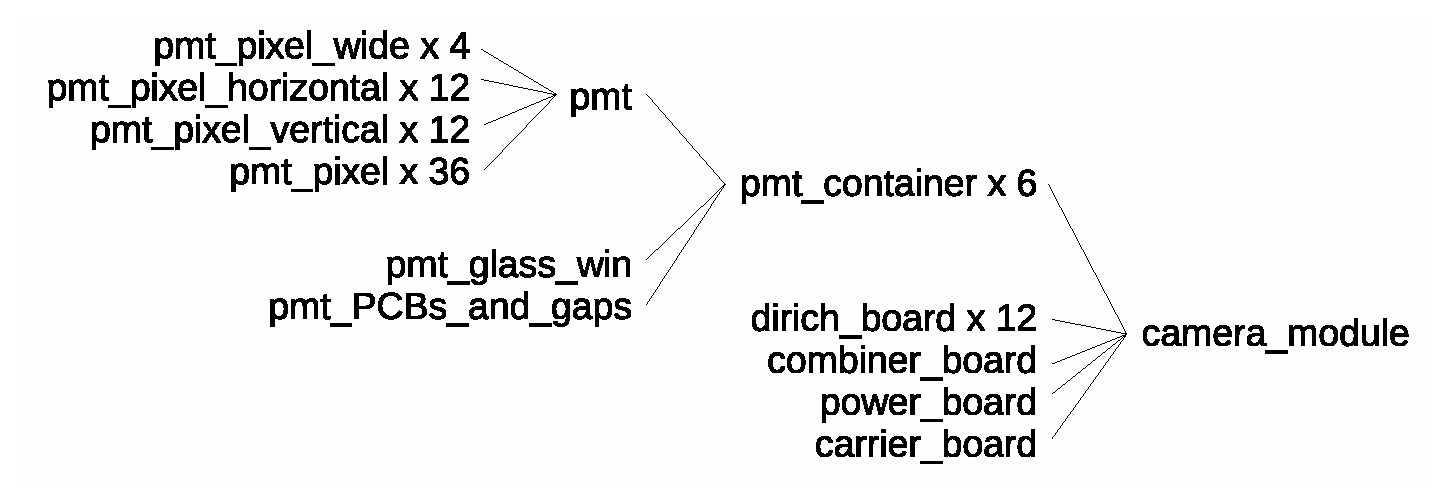
\includegraphics[width=0.7\textwidth]{pictures/Module_geoStructure.eps}
\caption{Иерархия объёмов, моделирующих модуль фоточувствительной камеры CBM RICH.}
\label{fig:Module_geoStructure}
\end{figure}